\chapter{Разработка рациональной конструкции БПЛА}

В этой главе рассматривается задача многодисциплинарного проектирования гипотетической конструкции БПЛА с крылом большого удлинения и с искривленной конструкцией центроплана.  Основной целью данной задачи является минимизация веса конструкции БПЛА при обеспечении необходимой прочности и жесткости и удовлетворении ограничениям на проектные параметры. При разработке конструкции учитывалось то обстоятельство, что некоторые ограничения на проектные параметры могли быть в дальнейшем легко изменены, а также предполагалась возможность дальнейшей вариации этих ограничений.

%удовлетворить ограничениям или ограничения? уточнить формулировку. (или обеспечить ограничения)

\section{Требования к конструкции БПЛА}


%В работе был рассмотрен ?вопрос проектировки? беспилотного летательного аппарата (БПЛА), предназаченного для длительного ($\approx24$~часа без дозаправки) барражирования в целях мониторинга и разведки (ограничения по режимам полета представлены на Рис.\ref{fig:ModeOfFlight}). В связи с этим к БПЛА были предъявлены высокие требования по малозаметности и аэродинамическому качеству. 




За основу гипотетической конструкции БПЛА была взята разработанная в ЦАГИ конструкция БПЛА, хорошо отвечающая требованиям высокого аэродинамического качества и требованиям малозаметности. Внешний вид гипотетической конструкции БПЛА показан на Рис.\ref{fig:BPLA_TSAGI}.
 

%Возможно, вставить пункт с геометрическими ограничениями
  
  



\begin{figure}[ht]
\centering
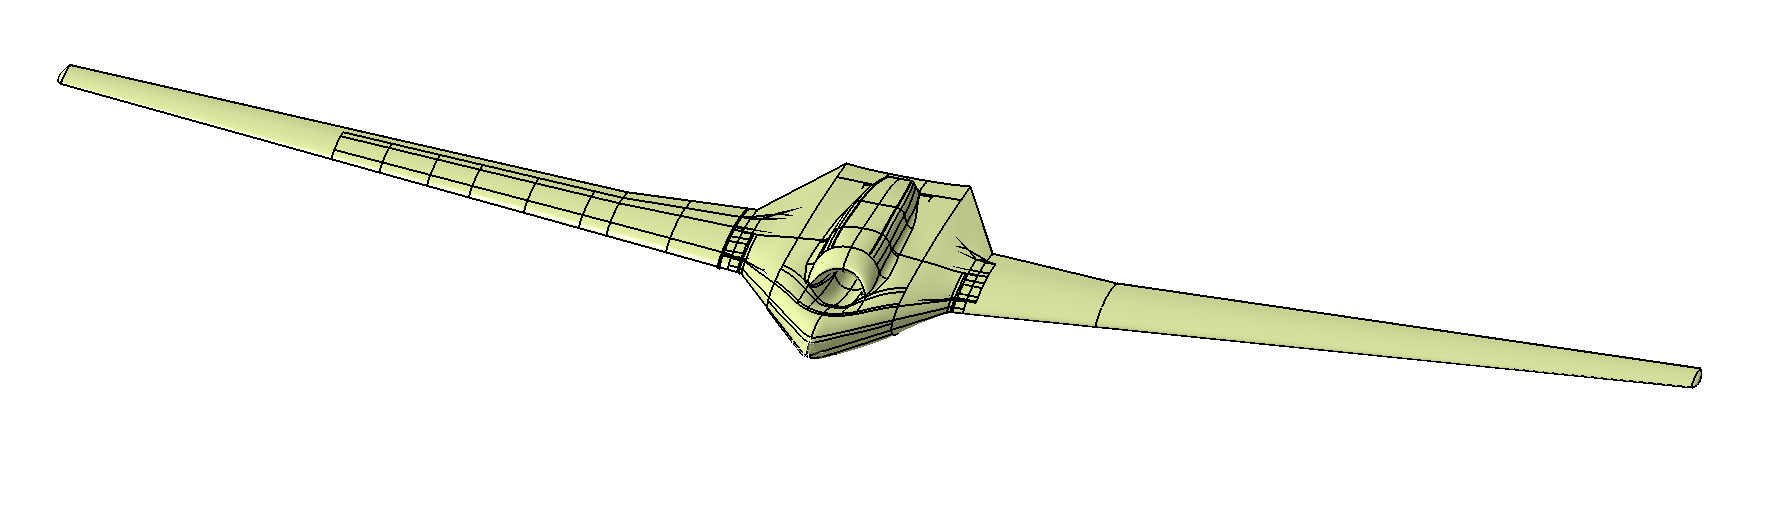
\includegraphics[width=1\textwidth]{BPS_Catia_Full}
\caption{Внешний вид гипотетической конструкции БПЛА}
\label{fig:BPLA_TSAGI}
\end{figure}

Конструкция выполнена по схеме ``бесхвостка'' с крылом большого удлинения и высокой степенью интегрированности крыла с фюзеляжем и двигателя с фюзеляжем. 

Для лучшей интеграции двигателя, включая воздухозаборник, в конструкцию БПЛА разработчикам пришлось использовать центроплан изогнутой формы (Рис.\ref{fig:OriginalSectionWithEngine}). Использование такой формы центроплана сопряжено с возможным возникновением новых проблем обеспечения прочности такого типа конструкции. Проблемы прочности в этом случае усугубляются из-за больших величин изгибающего момента, приходящего от крыла большого удлинения. 

Поскольку использование изогнутого центроплана может существенно ухудшить весовую эффективность БПЛА по сравнению с использованием прямого центроплана, для оценки величин этих весовых издержек необходимо проведение комплексных исследований по зависимости веса конструкции центроплана от геометрических параметров, характеризующих его кривизну. 
Необходимость таких исследований была связана с тем, что рассматриваемая в работе конструкция центроплана является нетрадиционной, и проведенный автором поиск конструкций прототипов не обнаружил наличия прямых прототипов данной конструкции центроплана для рассматриваемой размерности.

%Исследований центропланов такой формы ранее не проводилось.
 
%очевидно, что волнообразный центроплан может иметь напряжные вопросы с обеспечением прочности, т.к. такие центропланы в такой размерности не использовались, довольно нагружены. Сказать про компоновку, нарисовать её (общие вещи).

%с самого начала пишем, какие проблемы. Так сделали, такая компоновка, но у неё такие-то проблемы след волнообразный центроплан

%дальше: это может существенно ухудшить компоновку и весовую эффективность по сравнению с прямым центропланом. Цель работы - оценить возможные ухудшения. 

% и уже для того, чтобы оценить: следующий параграф 

Для оценки возможных ухудшений весовой эффективности конструкции центроплана необходимо построение расчетной прочностной модели гипотетической конструкции БПЛА, позволяющей проводить параметрический анализ зависимости прочности центроплана от геометрических параметров, определяющих его кривизну. Это необходимо и для последующего решения многодисциплинарной проектировочной задачи, в рамках которой будет возможность варьирования внешних аэродинамических обводов. 
Решение такой задачи предполагается осуществить в дальнейшем вне рамок данной работы. 

В настоящей (бакалаврской) работе не предполагается вариации внешних аэродинамических обводов и выхода этих параметров за пределы, определенные компоновкой "БПЛА-ЦАГИ", для которой они были выбраны из условия максимальной величины аэродинамического качества и минимума заметности, однако без учета требований прочности. 

%При построении модели необходимо было учесть ее дальнейшую модификацию, позволяющую варьировать форму внешних аэродинамических обводов. В бакалаврской работе форма внешних аэродинамических обводов постоянны. 


%Это скажем в разделе про нагрузки: Также постоянными считаются нагрузки на конструкцию (см.Раздел \ref{sec:externalLoads}). 

%В бакалаврской работе будем рассматривать только те обводы, которые есть в этой модели. И целью работы будет оценка потерь из-за такого центроплана (в прочности)

 
  
  

%Не забыть про то, что мы также хотим менять аэродинамику
%Требования: БПЛА, полет на таких-то высотах, столько-то. Весовая сводка такая-то, максимальные перегрузки, коэффициент запаса, аэродинамика. Ограничения - малозаметность, вес, пожаробезопасность отсека двигателя. 
%




\section{Компоновочная схема}
На рисунках 
\ref{fig:BPS_Catia_Top}--\ref{fig:BPS_Catia_Front} показана модель гипотетической конструкции БПЛА.


\begin{figure}[H]
\centering
\def\svgwidth{0.9\textwidth}
\input{figures/BPS_Catia_Top.pdf_tex}
\caption{Вид сверху}
\label{fig:BPS_Catia_Top}
\end{figure}

Как видно из рисунков для данной компоновочной схемы используется крыло большого удлинения. Из рисунка \ref{fig:BPS_Catia_WithoutSkin}, на котором представлена базовая конструктивно-силовая схема БПЛА, можно видеть, как происходит интеграция корпуса фюзеляжа, крыла и двигателя. 

\begin{figure}[H]
\centering
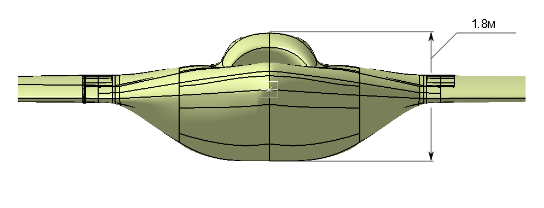
\includegraphics[width=0.8\textwidth]{BPS_Catia_Front}
\caption{Вид фюзеляжа спереди}
\label{fig:BPS_Catia_Front}
\end{figure}

\begin{figure}[H]
\centering
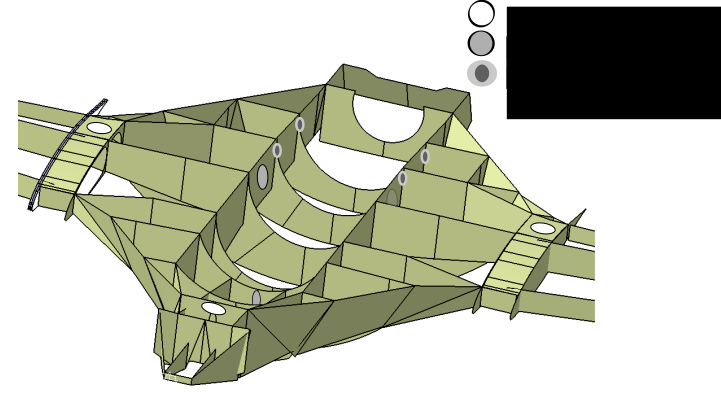
\includegraphics[width=0.8\textwidth]{BPS_Catia_WithoutSkin}
\caption{Вид фюзеляжа со снятой обшивкой}
\label{fig:BPS_Catia_WithoutSkin}
\end{figure}

%\begin{figure}[H]
%\centering
%\def\svgwidth{0.9\textwidth}
%\input{figures/BPS_Catia_WithoutSkin.pdf_tex}
%\caption{Вид фюзеляжа со снятой обшивкой с указанием узлов крепления шасси и двигателя}
%\label{fig:BPS_Catia_WithoutSkin}
%\end{figure}

Из рисунка видно, что двигатель с воздухозаборником значительно утоплены и находятся практически в середине фюзеляжа. Как уже отмечалось выше, эта особенность позволяет значительно улучшить малозаметность и аэродинамическое качество самолета (ссылка на отчет), но приводит к необходимости формировать искривленный центроплан. 

Формирование искривленного центроплана создает дополнительные проблемы из-за большой величины изгибающего момента в корне крыла. Еще одной проблемой обеспечения прочности корпуса БПЛА является высокая чувствительность параметров управляемости БПЛА от жесткостных характеристик корпуса и особенно зоны стыка крыла с центропланом, где расположены узлы крепления стоек основного шасси. Очевидно, что для решения проектировочной задачи необходимо проведение комплексных исследований прочности данной конструкции включая анализ прочности, устойчивости и управляемости. 

В данной схеме используется только горизонтальное оперение: руль высоты. Механизация крыла состоит из расщепляющихся элеронов на концах крыльев, элевонов и интерцепторов. В качестве тяги используется один реактивный двигатель, установленный в канале воздухозаборника. Места креплений стоек и замков шасси, расположение двигателя и узлов его крепления показаны на Рис. \ref{fig:BPS_Catia_Top_WithoutSkin}. 


\begin{figure}[H]
\centering
\def\svgwidth{0.9\textwidth}
\input{figures/BPS_Catia_Top_WithoutSkin.pdf_tex}
\caption{Вид сверху без обшивки с указанием узлов крепления шасси и двигателя}
\label{fig:BPS_Catia_Top_WithoutSkin}
\end{figure}

Отсеки фюзеляжа делятся на несколько групп по назначению. Распределение отсеков фюзеляжа по назначению представлено на Рис.\ref{fig:BPS_Catia_Top_PartRoles}. 

На рис.\ref{fig:BPS_Catia_Top_PartRoles} схематически показаны основные отсеки конструкции БПЛА. 

\begin{figure}[H]
\centering
\def\svgwidth{0.9\textwidth}
\input{figures/BPS_Catia_Top_PartRoles.pdf_tex}
\caption{Вид сверху с обозначением роли отсеков}
\label{fig:BPS_Catia_Top_PartRoles}
\end{figure}
	

\section{Внешние нагрузки}
\label{sec:externalLoads}
В работе исследуется прочность конструкции при случае нагружения A. Перегрузка $n_y = 2,97$, $M = 0,4$, скоростной напор $q = 503 \text{кгс}/\text{м}^2$, высота $H = 8\text{км}$. Нагрузки на конструкцию получены из работы \cite{BPS}, в которой были представлены расчетные нагрузки в диапазоне допускаемых режимов полета (см. Рис.\ref{fig:ModeOfFlight}). 
%описать режимы
Эпюры аэродинамических нагрузок представлены на Рис.\ref{fig:BendingMoments},\ref{fig:CuttingForces},\ref{fig:DistributedLoad}.



\begin{figure}[H]
\centering
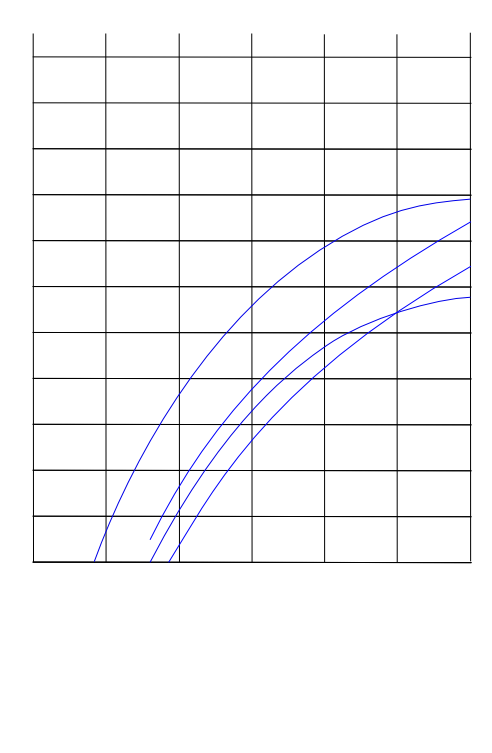
\includegraphics{HeightGraph}
\caption{Ограничения на режимы полета}
\label{fig:ModeOfFlight}
\end{figure}


\begin{figure}[H]
\centering
\def\svgwidth{0.7\textwidth}
\input{figures/BendingMoments.pdf_tex}
\caption{Эпюра изгибающих моментов}
\label{fig:BendingMoments}
\end{figure}

\begin{figure}[H]
\centering
\def\svgwidth{0.7\textwidth}
\input{figures/CuttingForces.pdf_tex}
\caption{Эпюра перерезывающих сил}
\label{fig:CuttingForces}
\end{figure}

\begin{figure}[H]
\centering
\def\svgwidth{0.7\textwidth}
\input{figures/DistributedLoad.pdf_tex}
\caption{Эпюра погонной нагрузки}
\label{fig:DistributedLoad}
\end{figure}

Как видно из имеющихся данных, влияние кручения на крыло невелико по сравнению с изгибом. В связи с этим в дальнейшем в работе будем пренебрегать кручением крыла, рассматривая только изгибные деформации. Где-то здесь будет график эпюры для кручения.




\section{Расчетные прочностные модели}
\section{Создание конечно-элементной модели проектируемого самолета}

В ходе работы были исследованы вопросы построения проектировочной модели БПЛА с крылом большого удлинения и несущим фюзеляжем. При помощи программного комплекса ``Conver'' (см. раздел \ref{sec:Conver}), исходя из концептуальной модели, предложенной конструкторами, была создана МКЭ-модель проектируемого БПЛА с исключенной верхней частью воздухозаборника, не несущей в себе силовых элементов. 

\begin{figure}[ht]
\centering
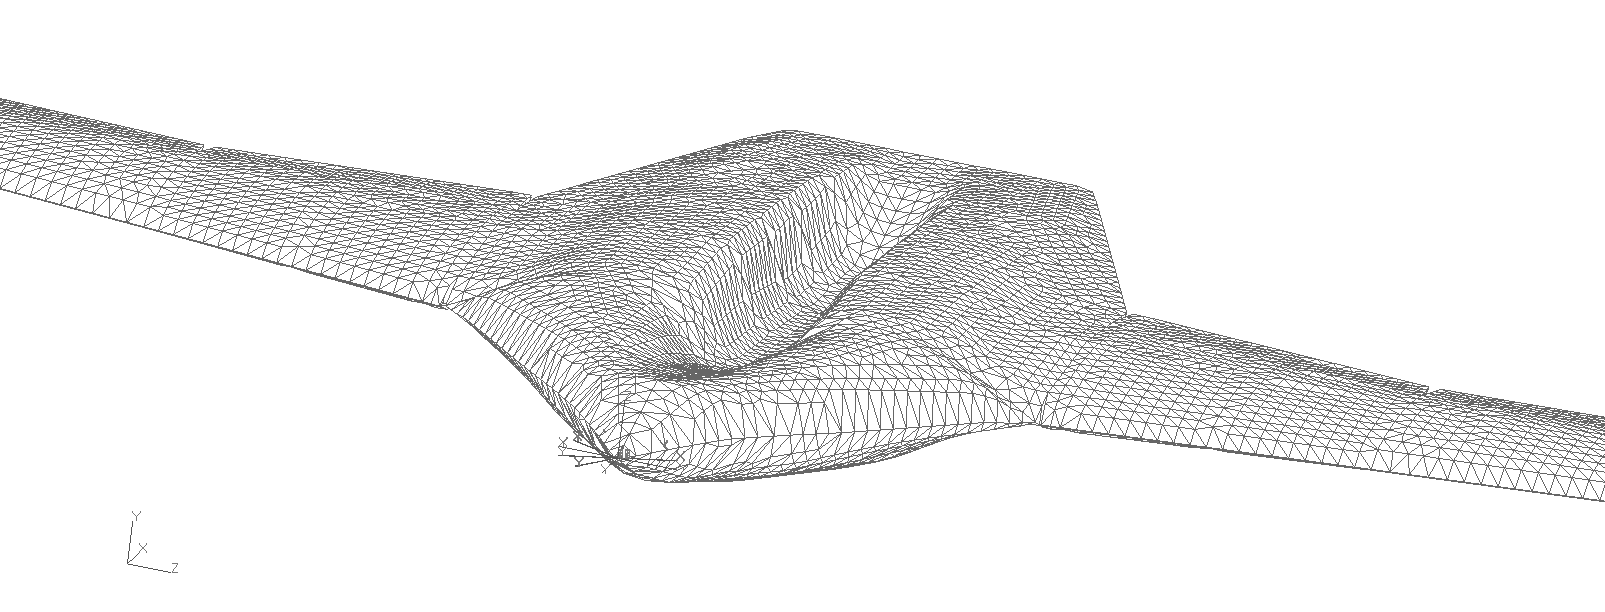
\includegraphics[width=0.8\textwidth]{BPLAfullModel}
\caption{МКЭ-модель проектируемого БПЛА без верхней части}
\label{fig:BPLAfullModel}
\end{figure}

\subsection{Подбор оптимальной дискретности модели}

В целях обеспечения точности расчета было проведено исследование зависимости напряженно-деформированного состояния самолета от максимального характерного размера конечных элементов, используемых в модели. 

С помощью программного комплекса ``Conver'' было построено 7 моделей самолета по одинаковой схеме с использованием различных размеров конечного элемента. Путем расчета моделей были определены средние величины напряжений для панелей и стенок в наиболее напряженных отсеках самолета (обозначены белым на  Рис.\ref{fig:WingRootPlain})

\begin{figure}[ht]
\centering
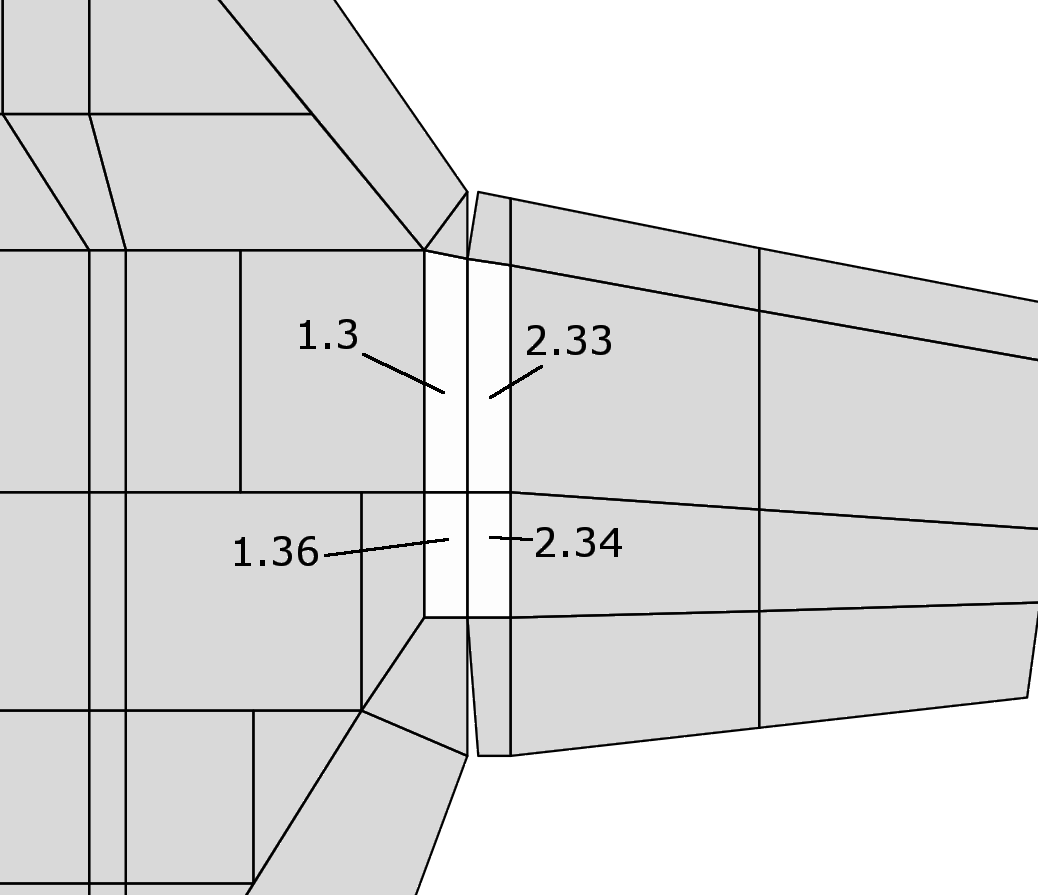
\includegraphics[width=0.5\textwidth]{RootOfWingWithSelectedPartsBW}
\caption{Схематичное изображение вида сверху в месте стыка правого крыла и фюзеляжа}
\label{fig:WingRootPlain}
\end{figure}




Исходя из полученных данных, была получена зависимость величины средних напряжений в панелях и стенках этих отсеков от выбора размера конечного элемента (Рис.\ref{fig:stressToDiscreteness})

\begin{figure}[ht]
\centering
%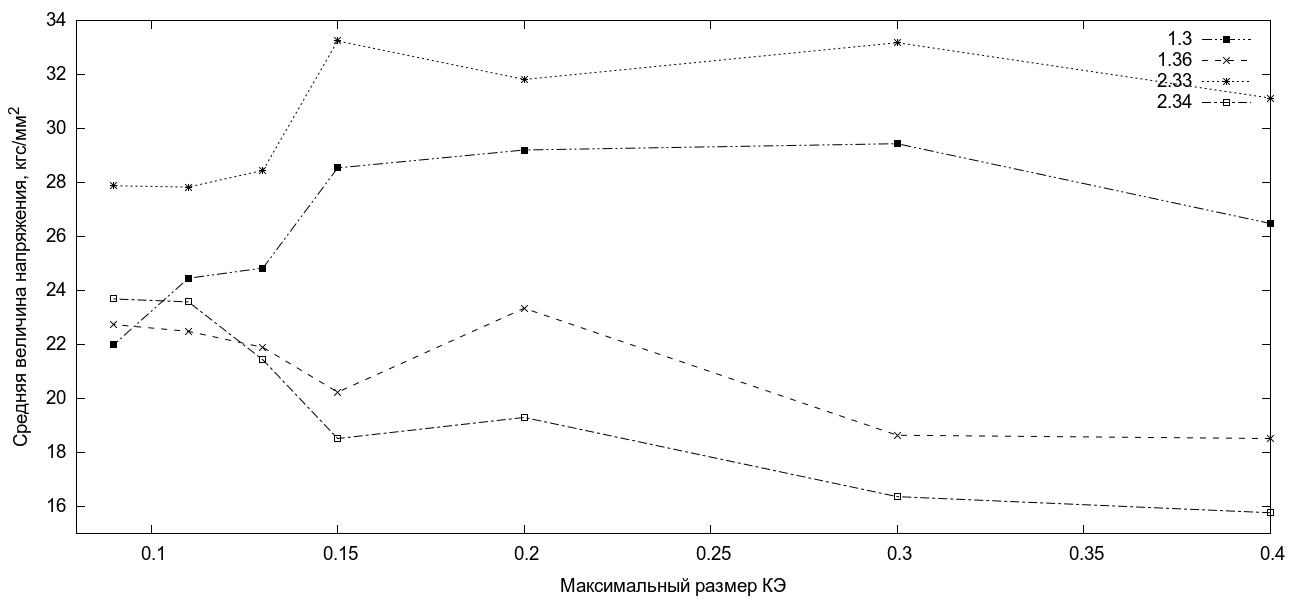
\includegraphics[width=0.8\textwidth]{StressToDiscretenessPlot}
% GNUPLOT: LaTeX picture with Postscript
\begingroup
  \makeatletter
  \providecommand\color[2][]{%
    \GenericError{(gnuplot) \space\space\space\@spaces}{%
      Package color not loaded in conjunction with
      terminal option `colourtext'%
    }{See the gnuplot documentation for explanation.%
    }{Either use 'blacktext' in gnuplot or load the package
      color.sty in LaTeX.}%
    \renewcommand\color[2][]{}%
  }%
  \providecommand\includegraphics[2][]{%
    \GenericError{(gnuplot) \space\space\space\@spaces}{%
      Package graphicx or graphics not loaded%
    }{See the gnuplot documentation for explanation.%
    }{The gnuplot epslatex terminal needs graphicx.sty or graphics.sty.}%
    \renewcommand\includegraphics[2][]{}%
  }%
  \providecommand\rotatebox[2]{#2}%
  \@ifundefined{ifGPcolor}{%
    \newif\ifGPcolor
    \GPcolorfalse
  }{}%
  \@ifundefined{ifGPblacktext}{%
    \newif\ifGPblacktext
    \GPblacktexttrue
  }{}%
  % define a \g@addto@macro without @ in the name:
  \let\gplgaddtomacro\g@addto@macro
  % define empty templates for all commands taking text:
  \gdef\gplbacktext{}%
  \gdef\gplfronttext{}%
  \makeatother
  \ifGPblacktext
    % no textcolor at all
    \def\colorrgb#1{}%
    \def\colorgray#1{}%
  \else
    % gray or color?
    \ifGPcolor
      \def\colorrgb#1{\color[rgb]{#1}}%
      \def\colorgray#1{\color[gray]{#1}}%
      \expandafter\def\csname LTw\endcsname{\color{white}}%
      \expandafter\def\csname LTb\endcsname{\color{black}}%
      \expandafter\def\csname LTa\endcsname{\color{black}}%
      \expandafter\def\csname LT0\endcsname{\color[rgb]{1,0,0}}%
      \expandafter\def\csname LT1\endcsname{\color[rgb]{0,1,0}}%
      \expandafter\def\csname LT2\endcsname{\color[rgb]{0,0,1}}%
      \expandafter\def\csname LT3\endcsname{\color[rgb]{1,0,1}}%
      \expandafter\def\csname LT4\endcsname{\color[rgb]{0,1,1}}%
      \expandafter\def\csname LT5\endcsname{\color[rgb]{1,1,0}}%
      \expandafter\def\csname LT6\endcsname{\color[rgb]{0,0,0}}%
      \expandafter\def\csname LT7\endcsname{\color[rgb]{1,0.3,0}}%
      \expandafter\def\csname LT8\endcsname{\color[rgb]{0.5,0.5,0.5}}%
    \else
      % gray
      \def\colorrgb#1{\color{black}}%
      \def\colorgray#1{\color[gray]{#1}}%
      \expandafter\def\csname LTw\endcsname{\color{white}}%
      \expandafter\def\csname LTb\endcsname{\color{black}}%
      \expandafter\def\csname LTa\endcsname{\color{black}}%
      \expandafter\def\csname LT0\endcsname{\color{black}}%
      \expandafter\def\csname LT1\endcsname{\color{black}}%
      \expandafter\def\csname LT2\endcsname{\color{black}}%
      \expandafter\def\csname LT3\endcsname{\color{black}}%
      \expandafter\def\csname LT4\endcsname{\color{black}}%
      \expandafter\def\csname LT5\endcsname{\color{black}}%
      \expandafter\def\csname LT6\endcsname{\color{black}}%
      \expandafter\def\csname LT7\endcsname{\color{black}}%
      \expandafter\def\csname LT8\endcsname{\color{black}}%
    \fi
  \fi
  \setlength{\unitlength}{0.0500bp}%
  \begin{picture}(8502.00,4534.00)%
    \gplgaddtomacro\gplbacktext{%
      \csname LTb\endcsname%
      \put(814,892){\makebox(0,0)[r]{\strut{} 16}}%
      \put(814,1267){\makebox(0,0)[r]{\strut{} 18}}%
      \put(814,1642){\makebox(0,0)[r]{\strut{} 20}}%
      \put(814,2017){\makebox(0,0)[r]{\strut{} 22}}%
      \put(814,2393){\makebox(0,0)[r]{\strut{} 24}}%
      \put(814,2768){\makebox(0,0)[r]{\strut{} 26}}%
      \put(814,3143){\makebox(0,0)[r]{\strut{} 28}}%
      \put(814,3518){\makebox(0,0)[r]{\strut{} 30}}%
      \put(814,3894){\makebox(0,0)[r]{\strut{} 32}}%
      \put(814,4269){\makebox(0,0)[r]{\strut{} 34}}%
      \put(1393,484){\makebox(0,0){\strut{} 0.1}}%
      \put(2512,484){\makebox(0,0){\strut{} 0.15}}%
      \put(3631,484){\makebox(0,0){\strut{} 0.2}}%
      \put(4749,484){\makebox(0,0){\strut{} 0.25}}%
      \put(5868,484){\makebox(0,0){\strut{} 0.3}}%
      \put(6986,484){\makebox(0,0){\strut{} 0.35}}%
      \put(8105,484){\makebox(0,0){\strut{} 0.4}}%
      \put(176,2486){\rotatebox{-270}{\makebox(0,0){\strut{}Средняя величина напряжения, $\text{кгс}/\text{мм}^2$}}}%
      \put(4525,154){\makebox(0,0){\strut{}Максимальный размер КЭ}}%
    }%
    \gplgaddtomacro\gplfronttext{%
      \csname LTb\endcsname%
      \put(7118,4096){\makebox(0,0)[r]{\strut{}$1.3$}}%
      \csname LTb\endcsname%
      \put(7118,3876){\makebox(0,0)[r]{\strut{}$1.36$}}%
      \csname LTb\endcsname%
      \put(7118,3656){\makebox(0,0)[r]{\strut{}$2.33$}}%
      \csname LTb\endcsname%
      \put(7118,3436){\makebox(0,0)[r]{\strut{}$2.34$}}%
    }%
    \gplbacktext
    \put(0,0){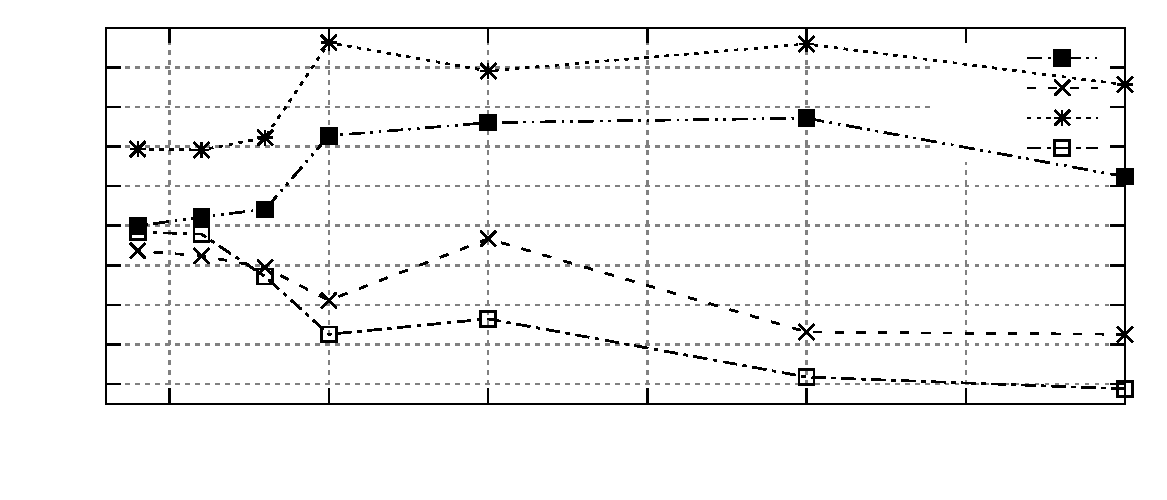
\includegraphics{StressToDiscreteness}}%
    \gplfronttext
  \end{picture}%
\endgroup

\caption{Зависимость средних напряжений в отсеках от величины КЭ}
\label{fig:stressToDiscreteness}
\end{figure}

На основании полученных данных и исходя из трудоемкости процесса расчета модели была определена оптимальная величина конечного элемента для дальнейшей работы над моделью, принятая равной $0,11\text{м}$. 
%Ниже приведены картины НДС в месте стыка крыла с фюзеляжем при различных размерах конечного элемента. 



\section{Результаты расчетов НДС конструкции БПЛА} 
\subsection{Проблемы проектирования}

В предложенной конструкторами схеме были выявлены некоторые проблемные места, в которых требовался дополнительный анализ. 

 \paragraph{Крепление хвостовой части к кессону центроплана} 
\label{sec:pants}
\begin{figure}[H]
\centering
\def\svgwidth{\textwidth}
\input{figures/IsoviewOfPants.pdf_tex}
%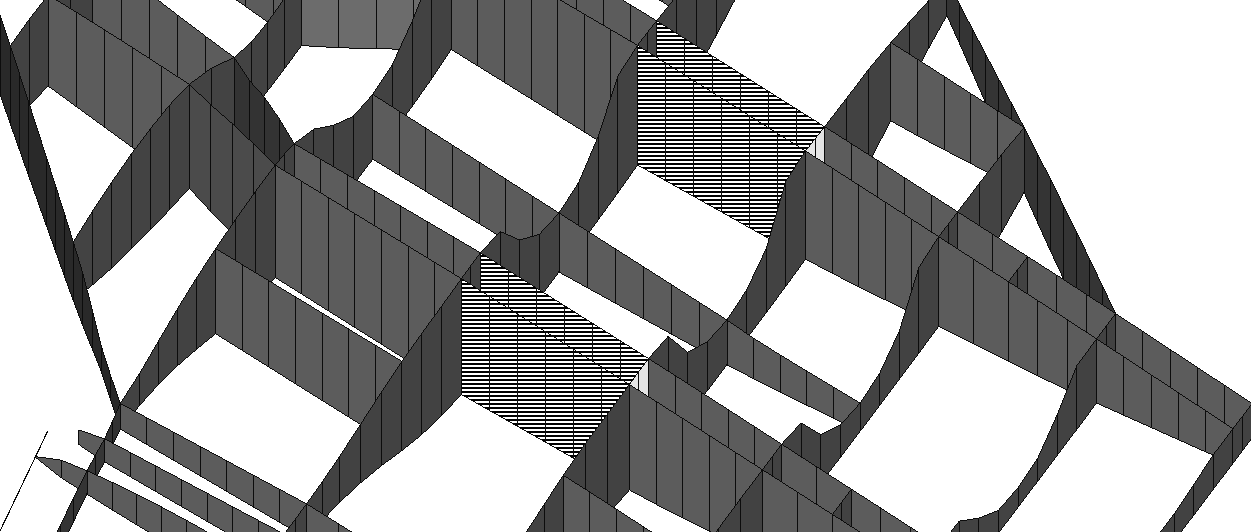
\includegraphics[width=0.6\textwidth]{IsoviewOfPantsBW}
\caption{Вид каркаса фюзеляжа}
\label{fig:IsoviewOfPants}
\end{figure}


Для частичной валидации решения, полученного в результате определния рациональных параметров (см. предыдущий раздел), была решена модельная задача по оценке устойчивости центральных стенок, обеспечивающих крепление хвостовой части гипотетического БПЛА к его центроплану (данные стенки обозначены на Рис.~\ref{fig:IsoviewOfPants} серой заливкой, светло-серой заливкой обозначены зоны основных узлов крепления двигателя). Эти стенки были нагружены перерезывающими усилиями, и необходима была проверка их по условиям устойчивости, которая не проводилась для этих элементов конструкции в процессе определения рациональных параметров. НДС стенок был оценен на основе аналитических формул. Схема нагружения модельных стенок показана на Рис.\ref{fig:IsoviewOfPantsModel}.

\begin{figure}[H]
\centering
%\def\svgwidth{0.9\textwidth}
\input{figures/IsoviewOfPantsModel.pdf_tex}
\caption{Схема нагружения модельных стенок}
\label{fig:IsoviewOfPantsModel}
\end{figure}

%
%\begin{figure}[H]
%\centering
%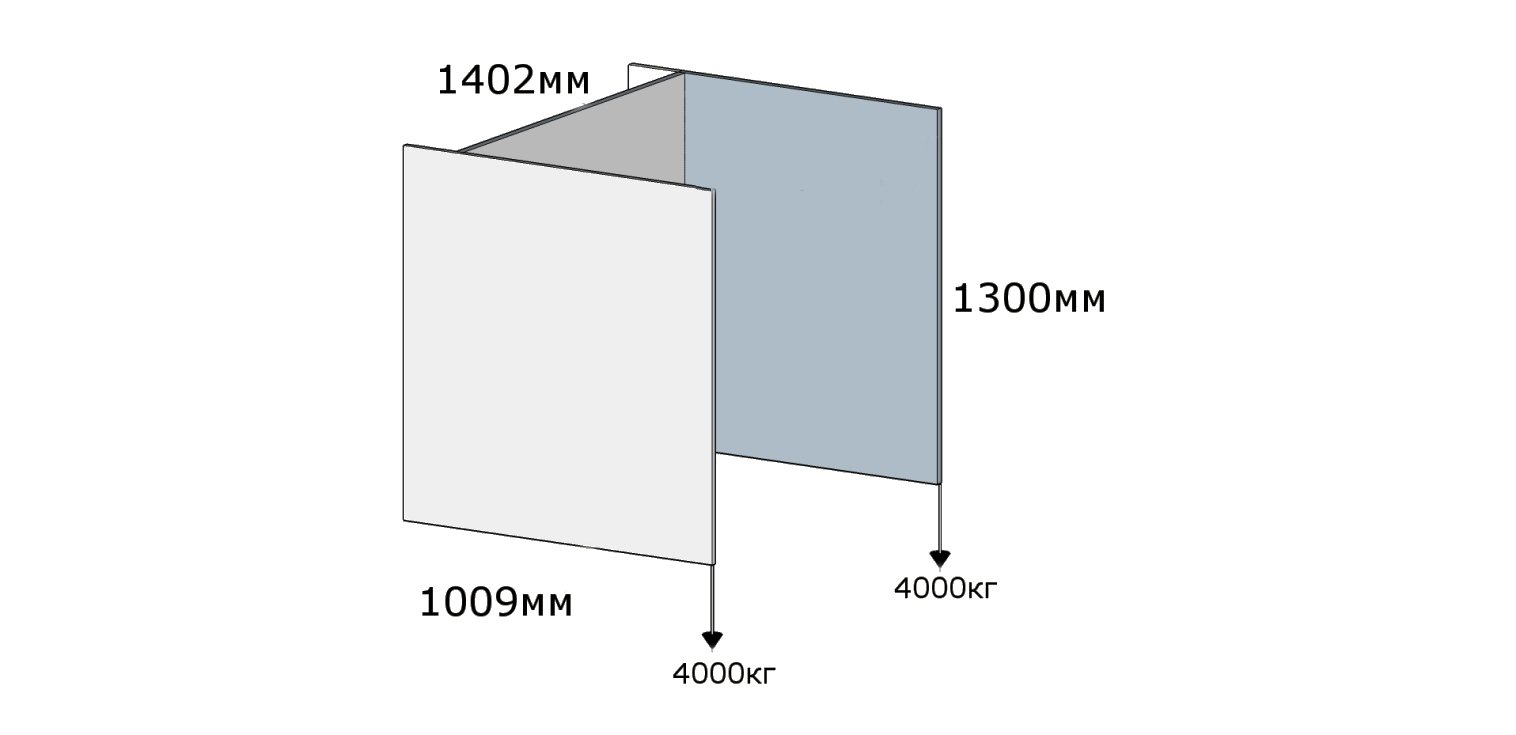
\includegraphics[width=0.8\textwidth]{IsoviewOfPantsModel}
%\caption{Схема нагружения модельных стенок}
%\label{IsoviewOfPantsModel}
%\end{figure}


Уровень нагружения был оценен по величинам касательных напряжений. Касательные напряжения в пластине при чистом сдвиге равны

\begin{equation}
\tau=\frac{3}{2}\cdot\frac{Q}{bh}
\end{equation}
Критические по устойчивости касательные напряжения в пластине при чистом сдвиге равны \cite{Volmir}:

\begin{equation}
\tau_\text{кр}=\frac{K}{12}\frac{\pi^2D}{b^2h} = \frac{K}{12}\frac{\pi^2E}{(1-\mu^2)}\left(\frac{h}{b}\right)^2,\, K=5.34 + 4\frac{a}{b},
\end{equation}
где $a$ - размер пластины вдоль направления действия силы, $b$ - размер пластины поперек направления действия силы, $h$ - толщина пластины, $D$ - изгибная жесткость пластины, $E$ - модуль Юнга, $\mu$ - модуль Пуассона материала пластины, $Q$ - приложенная сила.
Допускаемые толщины найдем из условия:

\begin{equation}
\tau_\text{кр} \geq \tau  
\end{equation}

\begin{equation}
h \geq \sqrt[3]{\frac{3\cdot12}{2}\frac{Qb\cdot(1-\mu^2)}{k\pi^2E}}
\end{equation}

Подставляя значения, получим:

\begin{equation}
Q=\frac{8000}{n}\text{кгс},\,a=1300\text{мм},\,b=1009\text{мм},\,\mu=0.3,\,E=7000\frac{\text{кгс}}{\text{мм}^2}
\end{equation}

\begin{equation}
h \geq \sqrt[3]{\frac{18\cdot8000\cdot1000\cdot(1-\mu^2)}{k\pi^2En}} = \frac{5.67}{\sqrt[3]{n}} 
\end{equation}

Таким образом, для случаев $n = 2$ и $n = 4$  были получены минимальные допустимые толщины, 
равные:

\begin{equation}
h\geq4.50\text{мм},\,n=2
\end{equation}
\begin{equation}
h\geq2.83\text{мм},\,n=4
\label{eq:pants_n4}
\end{equation}

Рациональные значения толщин исследуемых обшивок, полученные в данном проектировочном исследовании, оказались меньше ($h = 1\text{мм}$), чем приведенные в \ref{eq:pants_n4}. Таким образом, выполнение условий по устойчивости этих стенок привело к увеличению их толщин. Более рациональным способом увеличения сдвиговой жесткости этих стенок является использование ферменных подкрепляющих элементов.
\subsubsection{Фюзеляжная часть центроплана}

Другим проблемным местом была фюзеляжная часть центроплана. Из-за требований компоновки, а именно интеграции двигателя, центроплан необходимо делать изогнутым (Рис.\ref{fig:centroplan}). Это вносит дополнительные трудности в виде увеличения веса по сравнению с прямым центропланом. Исследованию фюзеляжной части центроплана (выделена серым на Рис.\ref{fig:centroplan}) посвящена глава \ref{chap:SolvingModel}.

\begin{figure}[ht]
\centering
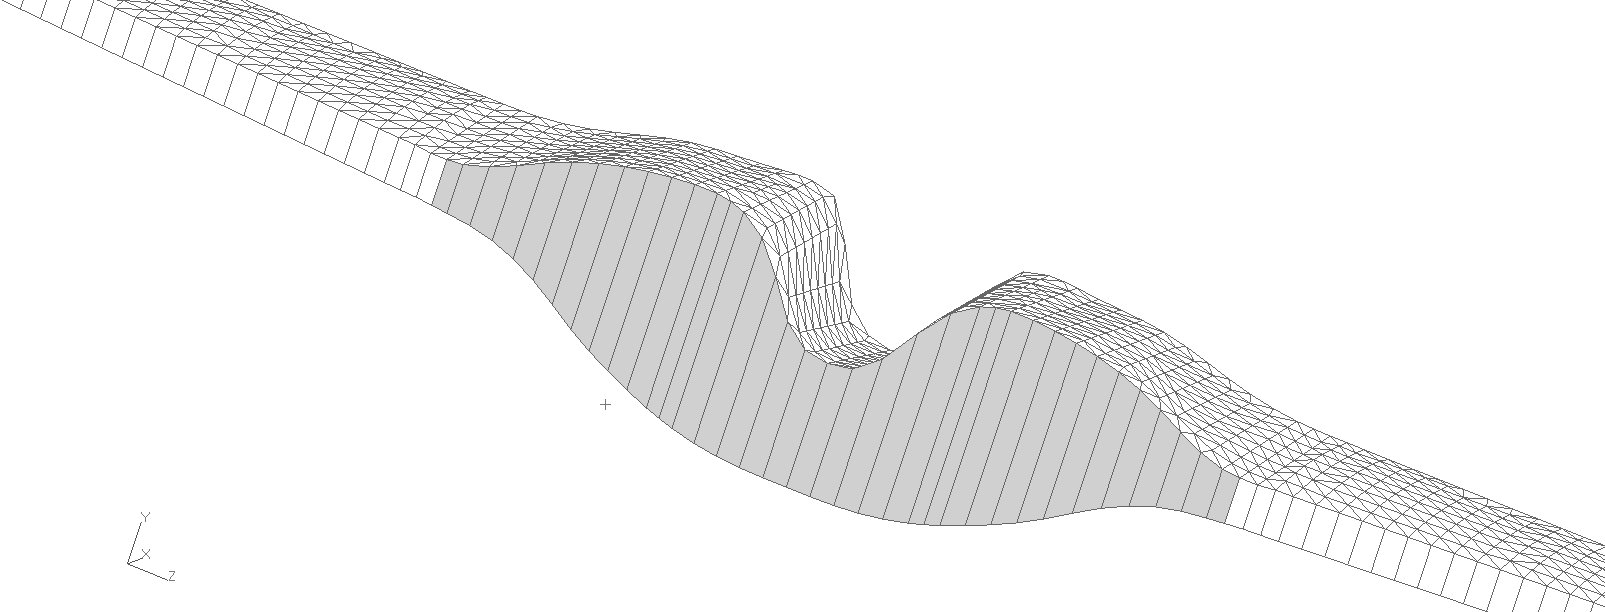
\includegraphics[width=0.6\textwidth]{centroplan}
\caption{Изогнутый центроплан с выделением исследуемой части}
\label{fig:centroplan}
\end{figure}


\section{Рациональные параметры КСС фюзеляжа}
На основе полученных в разделе \ref{sec:creationOfOneModel} данных была проведена оптимизация толщин стенок отсеков и панелей для выполнения требований прочности конструкции. Эпюры толщин верхних и нижних панелей центроплана, а также эпюры погонных усилий $N_1$ в верхних и нижних панелях центроплана представлены на Рис. \ref{fig:epures}

\begin{figure}[H]
\centering
\captionsetup{justification=centering}
\begin{subfigure}[b]{0.49\textwidth}
	\centering
	\def\svgwidth{\textwidth}
	\footnotesize
	\input{figures/EpureDistributedLoadN1Top.pdf_tex}	
	\normalsize
	%\label{fig:epureloadn1top}
	\caption{Эпюра погонных усилий $N_1$ в верхних панелях центроплана}
\end{subfigure}
\begin{subfigure}[b]{0.49\textwidth}
	\centering
	\def\svgwidth{\textwidth}
	\input{figures/EpureDistributedLoadN1Bottom.pdf_tex}
	%\label{fig:epureloadn1bottom}
	\caption{Эпюра погонных усилий $N_1$ в нижних панелях центроплана}
\end{subfigure}
\begin{subfigure}[b]{0.49\textwidth}
	\centering
	\def\svgwidth{\textwidth}
	\input{figures/EpureDistributedWeightTop.pdf_tex}
	%\label{fig:epureweighttop}
	\caption{Эпюра погонного веса верхних панелей центроплана}
\end{subfigure}
\begin{subfigure}[b]{0.49\textwidth}
	\centering
	\def\svgwidth{\textwidth}		\input{figures/EpureDistributedWeightBottom.pdf_tex}
	%\label{fig:epureweightbottom}
	\caption{Эпюра погонного веса нижних панелей центроплана}
\end{subfigure}
	\caption{Эпюры погонных усилий $N_1$ и погонного веса для верхних и нижних панелей центроплана}
	\label{fig:epures}
\end{figure}
%
%
%\begin{figure}[H]
%\centering
%\begin{subfigure}[b]{0.7\textwidth}
%	\centering
%	\def\svgwidth{\textwidth}
%	\input{figures/EpureDistributedLoadN2Top.pdf_tex}
%	\label{fig:epure:loadn2top}
%	\caption{Верхние панели}
%\end{subfigure}
%\begin{subfigure}[b]{0.7\textwidth}
%	\centering
%	\def\svgwidth{\textwidth}	\input{figures/EpureDistributedLoadN2Bottom.pdf_tex}
%	\label{fig:epure:loadn2bottom}
%	\caption{Нижние панели}
%\end{subfigure}
%\label{fig:epure:loadn2}
%\caption{Эпюра $N_y$}
%\end{figure}
%
%\begin{figure}
%	\centering
%	\def\svgwidth{\textwidth}
%	\input{figures/EpureDistributedLoadN12Bottom.pdf_tex}
%	\label{fig:epure:loadn12bottom}
%	\caption{Эпюра $N_\text{xy}$. Нижние панели}
%\end{figure}
%
%\begin{figure}
%	\centering
%	\def\svgwidth{\textwidth}
%	\input{figures/EpureDistributedLoadN12Top.pdf_tex}
%	\label{fig:epure:loadn12top}
%	\caption{Эпюра $N_\text{xy}$. Верхние панели}
%\end{figure}



%Параметры оптимизированной модели представлены в таблице \ref{tab:paramsOfOptimizedScheme}

%Остальные две главы будут как приложение к этой мощной главе: исследование влияния искривления кессона центроплана на его вес, выбор рациональной КСС.

